\phantomsection
\addcontentsline{toc}{subsection}{Δομή βάσης δεδομένων}
\subsection*{Δομή βάσης δεδομένων}

% ========================================

\textbf{Πίνακας "sessions"}

Αντιπροσωπεύει μία είσοδο ενός παίκτη στο παιχνίδι. Μπορεί να είναι ο ίδιος πραγματικός παίκτης, είτε με διαφορετικό, είτε με το ίδιο όνομα χρήστη. Οι στήλες του πίνακα είναι οι εξής:

\begin{itemize}
    \item \textbf{id:} Το μοναδικό id κάθε session
    \item \textbf{username:} Το μή-μοναδικό όνομα χρήστη
    \item \textbf{created\_at:} Η ημερομηνία και ώρα δημιουργίας του session
\end{itemize}

% ========================================

\vspace{5mm}
\textbf{Πίνακας "time\_trials"}

Αποθηκεύει πληροφορίες για κάθε επιτυχή προσπάθεια παίκτη στη δυσκολία με χρονομέτρηση. Ο πίνακας αυτός χρησιμοποιείται σαν πίνακας σκορ, ο οποίος εμφανίζεται στους παίκτες. Οι στήλες του πίνακα είναι οι εξής:

\begin{itemize}
    \item \textbf{id:} Το μοναδικό id της κάθε εγγραφής
    \item \textbf{type:} Ο αλγόριθμος τον οποίο αφορά η εγγραφή (π.χ. Bubble Sort)
    \item \textbf{time:} Ο χρόνος στον οποίο ολοκληρώθηκε η προσπάθεια (σε milliseconds)
    \item \textbf{number\_of\_values:} Ο αριθμός των κουτιών όταν έγινε η προσπάθεια
    \item \textbf{required\_moves:} Ο ελάχιστος αριθμός κινήσεων που χρειαζόταν για την ταξινόμηση των αρχικών τιμών
    \item \textbf{created\_at:} Η ημερομηνία και ώρα που ολοκληρώθηκε η προσπάθεια
\end{itemize}

Ο στόχος των στηλών \textbf{number\_of\_values} και \textbf{required\_moves} είναι έτσι ώστε τα σκορ που εμφανίζονται στους παίκτες να είναι σχετικά με αυτά που χρειάζονται να κάνουν οι ίδιοι. Για παράδειγμα αν ένας παίκτης παίζει το παιχνίδι με 10 κουτιά δεν είναι σωστό να εμφανίζονται τα τοπ σκορ παικτών που έχουν γίνει με 5 κουτιά.

% ========================================

\vspace{5mm}
\textbf{Πίνακας "container\_interactions"}

Ο πίνακας αυτός αποθηκεύει κάθε αλληλεπίδραση ενός παίκτη με κάποιο κουτί. Μέσω αυτού του πίνακα μπορεί κάποιος να βρει κάθε κίνηση που έχει κάνει ένας παίκτης σε οποιαδήποτε στιγμή κατά τη διάρκεια του παιχνιδιού του.

\begin{itemize}
    \item \textbf{id:} Το μοναδικό id της κάθε εγγραφής
    \item \textbf{container\_index:} Η θέση του κουτιού στη λίστα με όλα τα κουτιά
    \item \textbf{received\_value:} Η τιμή που ο παίκτης πήρε από το κουτί
    \item \textbf{placed\_value:} Η τιμή που ο παίκτης άφησε στο κουτί
    \item \textbf{is\_valid:} Εάν η κίνηση είναι σωστή η λάθος
    \item \textbf{container\_values:} Οι τιμές όλων των κουτιών αμέσως μετά την αλληλεπίδραση του παίκτη
    \item \textbf{algorithm\_type:} Ο αλγόριθμος τον οποίο αφορά η εγγραφή (π.χ. Bubble Sort)
    \item \textbf{game\_mode:} Η επιλεγμένη δυσκολία (Guided, Time Trial)
    \item \textbf{created\_at:} Η ημερομηνία και ώρα που έγινε η αλληλεπίδραση
    \item \textbf{session\_id:} Το μοναδικό id του παίκτη που έκανε την αλληλεπίδραση
\end{itemize}

% ========================================

\vspace{5mm}
\textbf{Πίνακας "logs"}

Ο πίνακας αποθηκεύει πληροφορίες για κάθε κίνηση του παίκτη μέσα στο παιχνίδι, εκτός από τις αλληλεπιδράσεις με τα κουτιά. Εγγραφές σε αυτό το πίνακα δημιουργούνται όταν ένας παίκτης δημιουργεί ή κλείνει έναν κόσμο, όταν ξεκινά ένα παιχνίδι και όταν είναι επιτυχής ή αποτυχής σε μία προσπάθεια του.

\begin{itemize}
    \item \textbf{id:} Το μοναδικό id της κάθε εγγραφής
    \item \textbf{type:} Ο τύπος του log (Game Won, Game Over, etc.)
    \item \textbf{message:} Ένα μήνυμα που περιγράφει το log
    \item \textbf{algorithm\_type:} Ο αλγόριθμος τον οποίο αφορά η εγγραφή (π.χ. Bubble Sort)
    \item \textbf{game\_mode:} Η επιλεγμένη δυσκολία (Guided, Time Trial)
    \item \textbf{container\_values:} Οι τιμές όλων των κουτιών τη στιγμή του log
    \item \textbf{created\_at:} Η ημερομηνία και ώρα του log
    \item \textbf{session\_id:} Το μοναδικό id του παίκτη που έκανε το log
\end{itemize}

% ========================================

\vspace{5mm}
\textbf{Πίνακας "algorithms"}

Ο πίνακας αυτός περιέχει ρυθμίσεις για τους αλγόριθμους μέσα στο παιχνίδι. Εδώ βρίσκονται οι ρυθμίσεις για τον αριθμό των κουτιών που εμφανίζονται για τον εκάστοτε αλγόριθμο, καθώς και λοιπές ρυθμίσεις τους. Οι τιμές αυτές αλλάζουν μέσω της διαχειριστικής διεπαφής που έχουν πρόσβαση οι εκπαιδευτικοί.

\begin{itemize}
    \item \textbf{id:} Το μοναδικό id της κάθε εγγραφής
    \item \textbf{type:} Ο αλγόριθμος τον οποίο αφορούν οι ρυθμίσεις (π.χ. Bubble Sort)
    \item \textbf{number\_of\_values:} Ο αριθμός των κουτιών που θα εμφανιστούν
    \item \textbf{min\_value:} Η μικρότερη τιμή που μπορεί να εμφανιστεί σε κουτί
    \item \textbf{max\_value:} Η μεγαλύτερη τιμή που μπορεί να εμφανιστεί σε κουτί
    \item \textbf{created\_at:} Η ημερομηνία και ώρα που δημιουργήθηκαν οι ρυθμίσεις
    \item \textbf{updated\_at:} Η ημερομηνία και ώρα που άλλαξαν τελευταία φορά οι ρυθμίσεις
\end{itemize}

% ========================================

\textbf{Σχεσιακό διάγραμμα}

\begin{figure}[H]
    \centering
    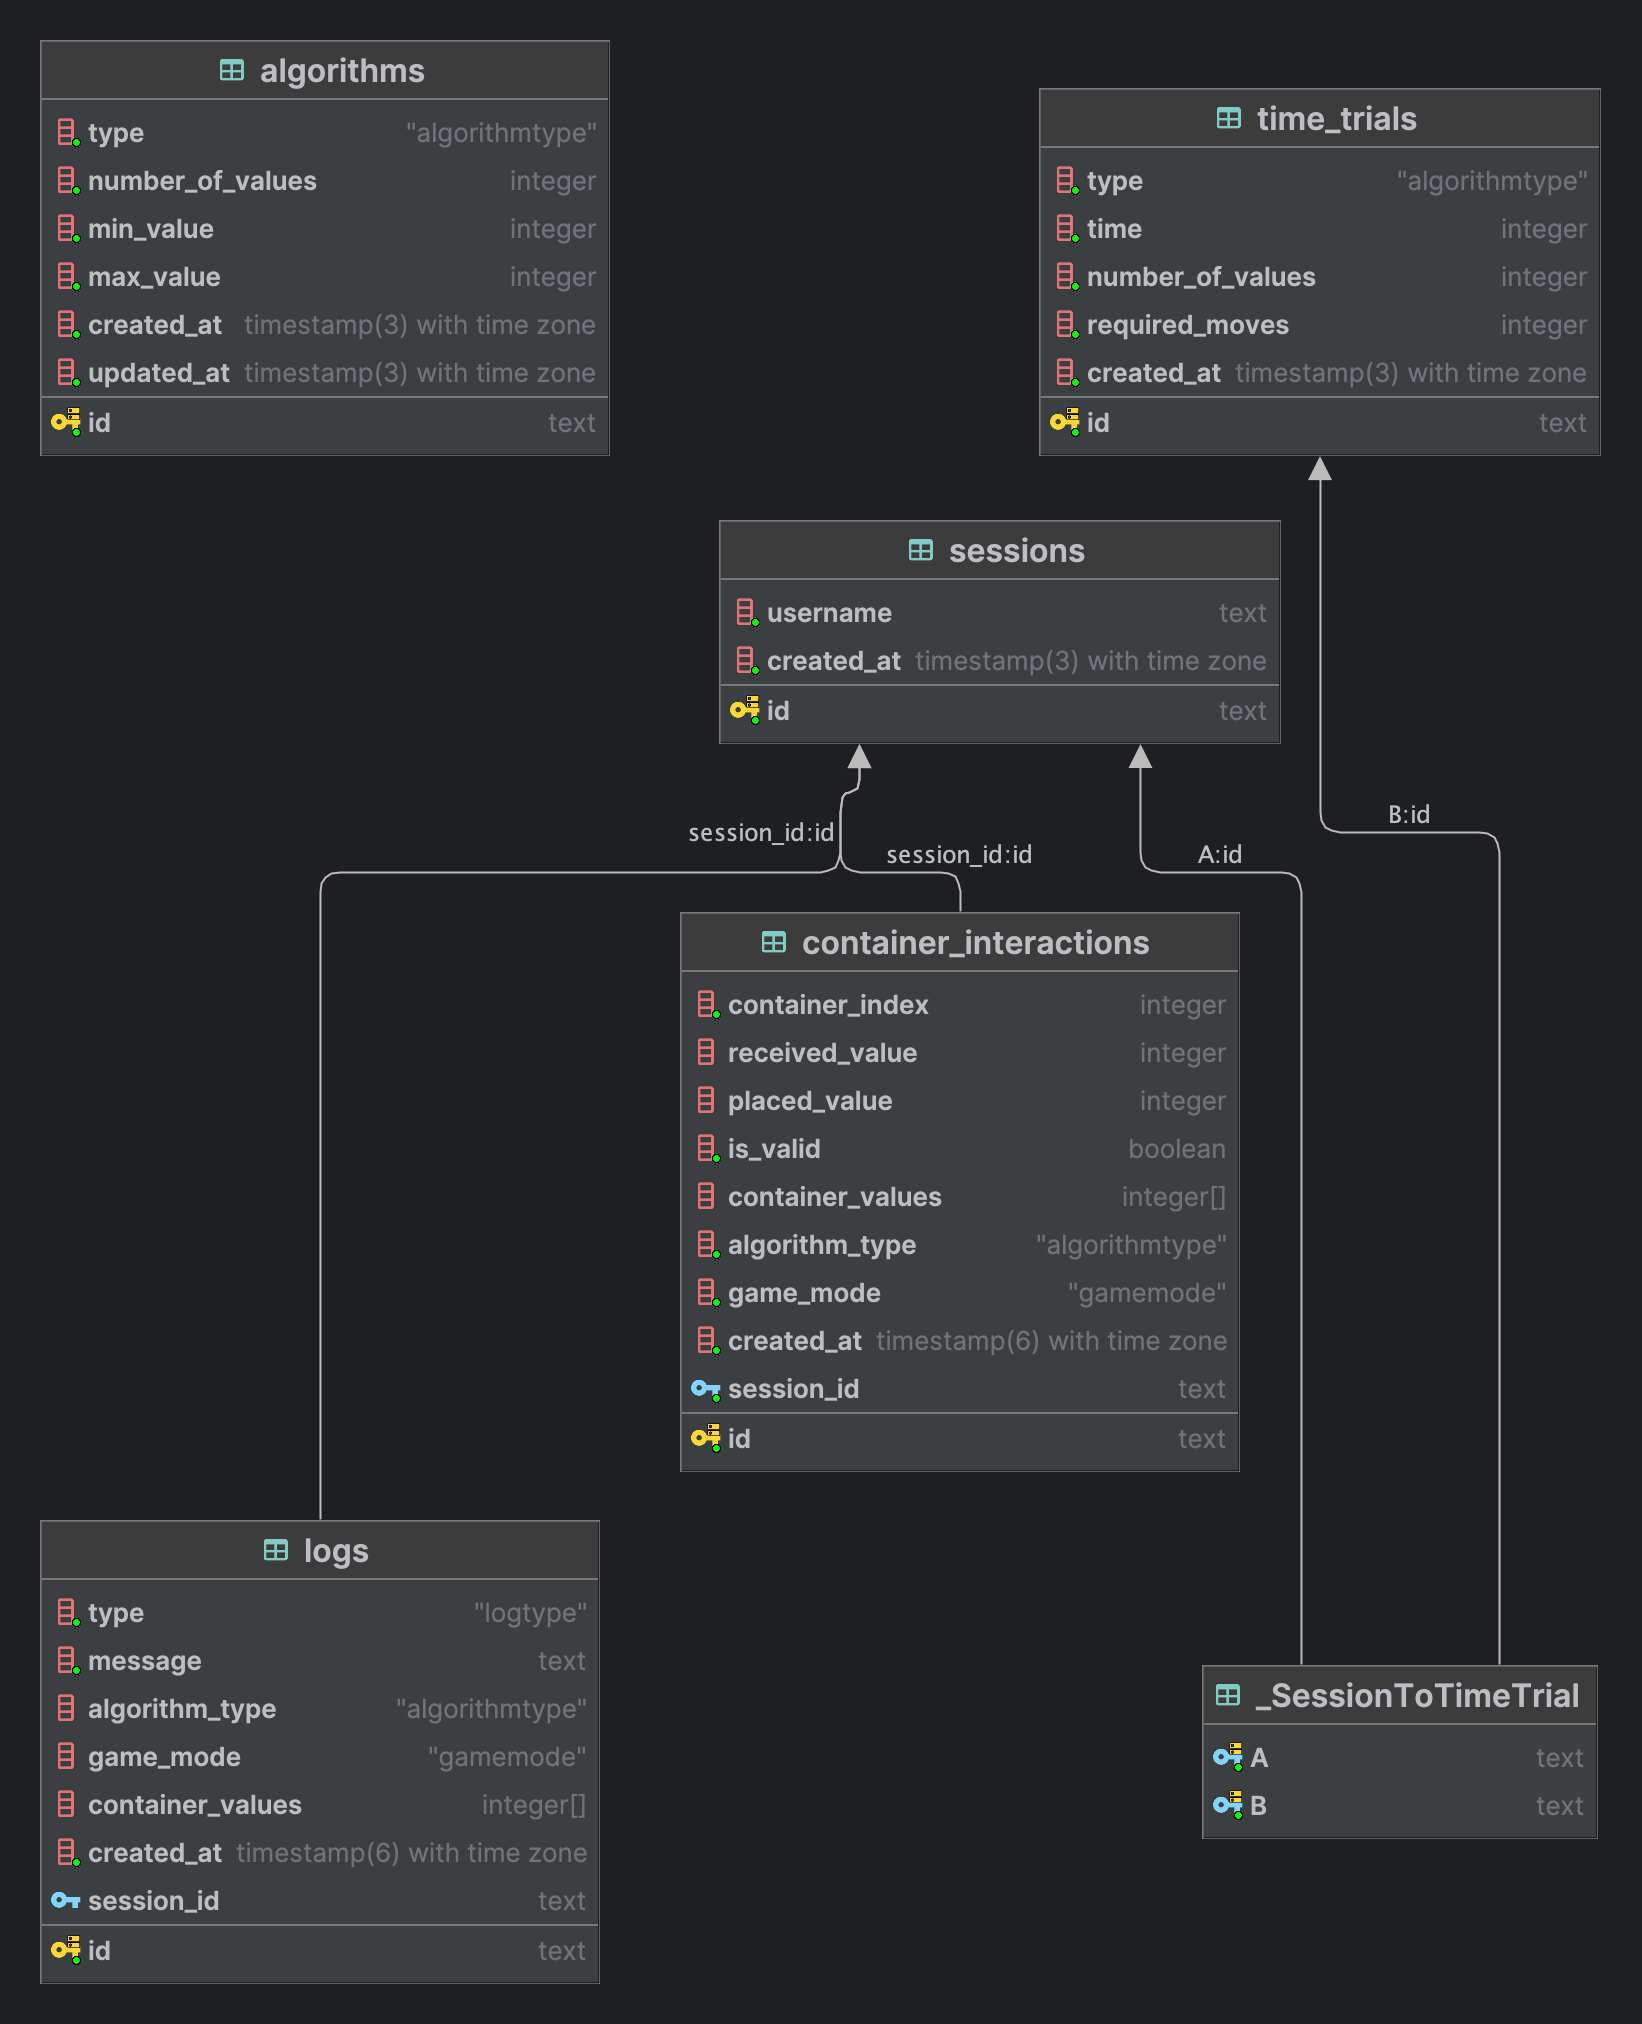
\includegraphics[width=0.8\linewidth]{sections/appendices/a/images/db_schema}
    \caption{Σχεσιακό διάγραμμα της βάσης δεδομένων}
    \label{fig:db_schema}
\end{figure}
